\chapter*{\thechapter \quad Git}
\addcontentsline{toc}{chapter}{\thechapter \quad Git}
\paragraph{}

A lógica para a execução do projeto foi a seguinte:
\begin{itemize}
    \item Inicialmente foi criada a estrutura de grande parte do projeto por parte do Responsável de repositório e esta foi colocada disponivel na branch main do repositório;
    \item Todos os contribuidores fizeram clone do projeto nos seus computadores.;
    \item Desse ponto em diante foi utilizada sempre a mesma lógica por parte dos contribuidores:
    \begin{itemize}
    \item Criação de uma branch;
    \item Alterações do conteúdo da respetiva branch;
    \item Commit das alterações feitas;
    \item Criação de um pull request do branch criado para a main;
    \end{itemize}
    
    \item Para um Complete de um Pull Request é necessário:
    \begin{itemize}
    \item Aprovação por parte dos contribuidores;
    \item Complete por parte do responsavel do repositório;
    \end{itemize}
\end{itemize}

\begin{table}
\begin{center}
\begin{tabular}{||c c||} 
 \hline
 Responsáveis de repositório & Contribuidores  \\ [0.5ex] 
 \hline\hline
 António Ferreira & António Ferreira \\ 
 \hline
  & Diogo Miranda \\
 \hline
  & Pedro Meneses \\
 \hline
  & Ricardo Fernandes \\ [1ex] 
 \hline
\end{tabular}
\caption{Tabela de responsabilidades}
\label{table: Tabela de responsabilidades}
\end{center}
\end{table}



\begin{figure}[H]
	\begin{center}
		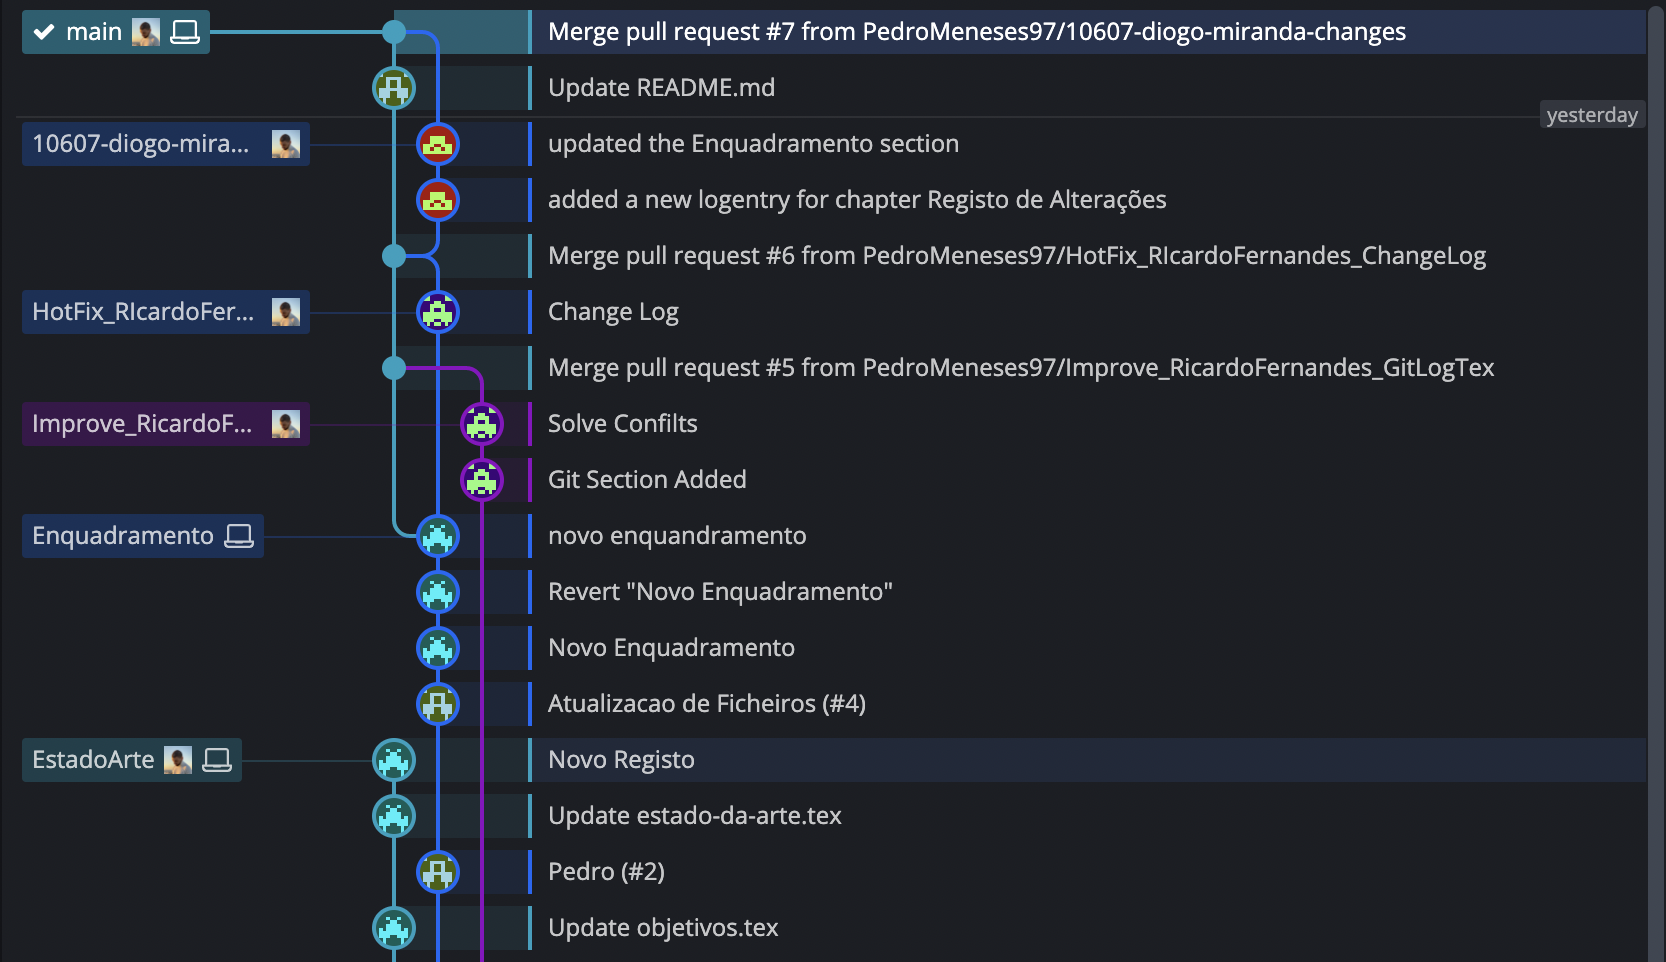
\includegraphics[width=0.66\textwidth]{chapter/image/git1.png}
	\end{center}
		\caption{Fotografia de Git}
		\label{fig:viaconsulting-sophos-pic1}
\end{figure}



\begin{figure}[H]
	\begin{center}
		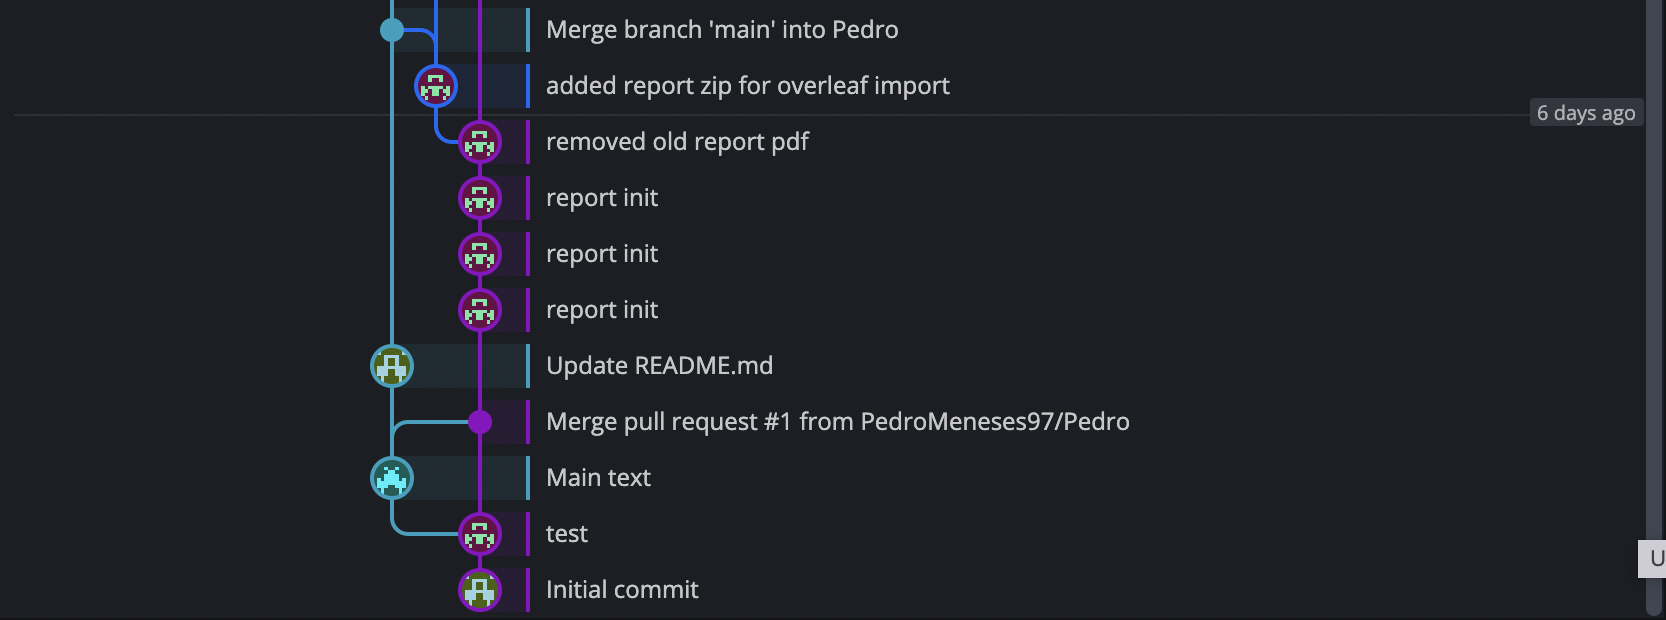
\includegraphics[width=0.66\textwidth]{chapter/image/git2.png}
	\end{center}
		\caption{Git 2}
		\label{fig:viaconsulting-sophos-pic1}
\end{figure}



\begin{figure}[H]
	\begin{center}
		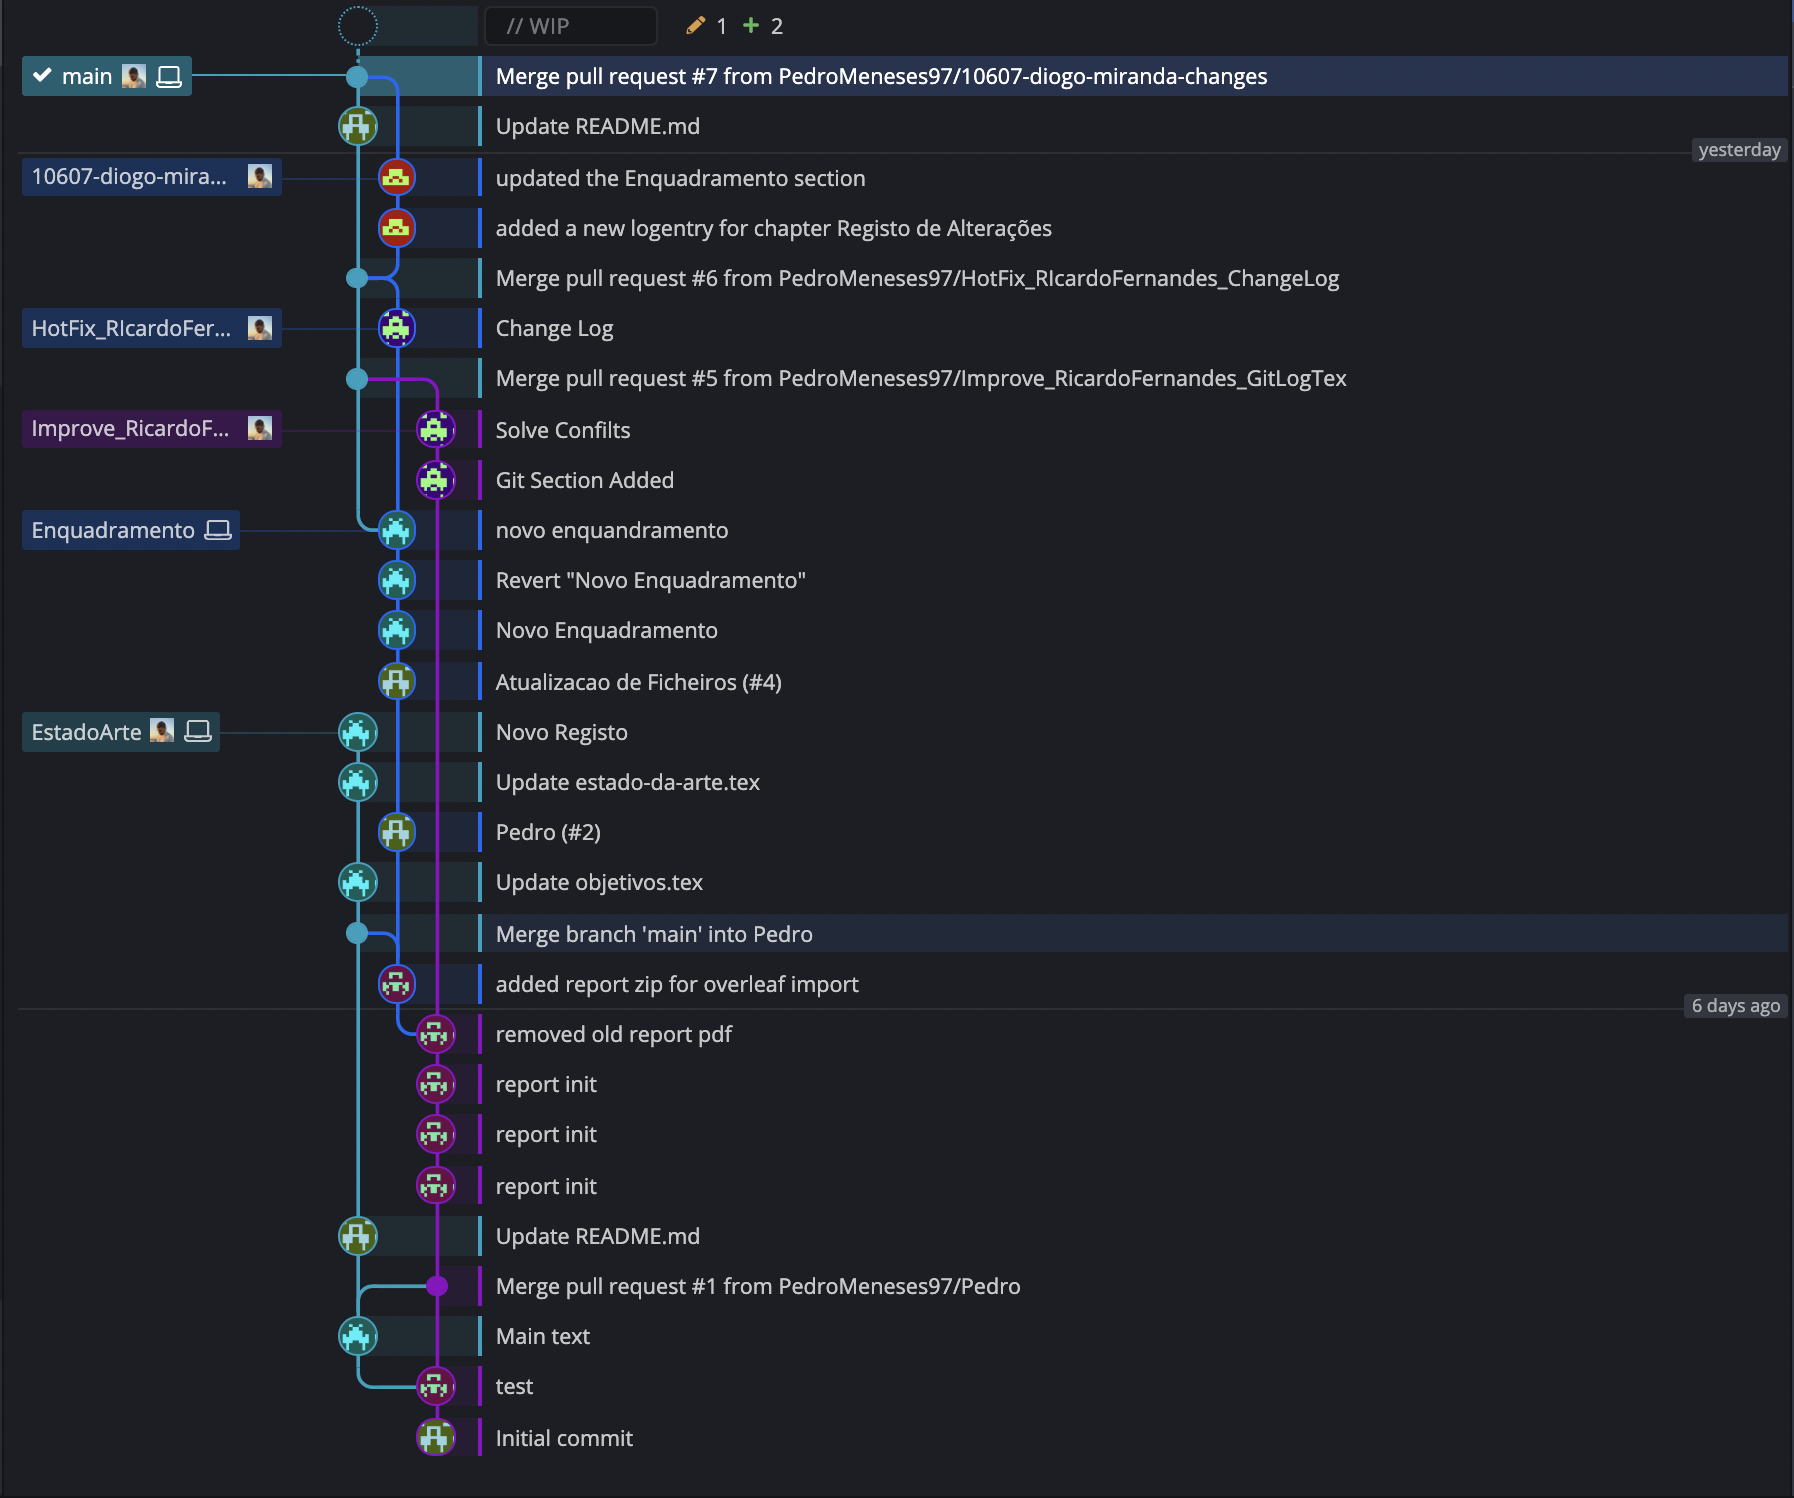
\includegraphics[width=0.66\textwidth]{chapter/image/git3.png}
	\end{center}
		\caption{Full Git}
		\label{fig:viaconsulting-sophos-pic1}
\end{figure}

